\section{Традиционные подходы в организации жилища и адаптация к условиям Арктики}\label{CH01_experience_indigenous}
Объективную оценку степени экстремальности, <<суровости>>, окружающей среды возможно произвести по нескольким показателям, среди которых авторы выделяют:

\begin{itemize}
    \item продолжительность отопительного периода, выражаемое в градус-сутках отопительного периода (ГСОП);
    \item наличие доступа к пригодной для питья воды, выражаемое в м³/км расстояния до источника;
    \item наличие и доступность пригодного для дыхания кислорода, выражаемое в м³/час;
    \item стоимости доставки грузов, у.е./км;
    \item продолжительность естественной освещённости, выражаемая в часах;
\end{itemize}


Традиционные, выработанные веками коренным (местным) населением объемно-планировочные решения в строительстве жилища и хозяйственных построек,
продиктованных проживанием в экстремальных природно-климатических условиях Арктики, направлены на адаптацию к таковым условиям.

Коренные жители арктических районов в основу быта преимущественно ставили скотоводство, основанное на разведении оленей, береговые поселенцы, такие как чукчи,
эскимосы и коряки практиковали также морской зверобойный промысел. Оленеводам был свойственен кочевой образ жизни, причем перемещались они по определенным традиционно
складывающимся маршрутам каслания (выпаса стада на протяжении сезона) оленей, которые мигрировали по мере поедания растущего на пастбищах ягеля. Селения-стойбища оленеводов
могли обустраиваться на новых местах с периодичностью в несколько дней или недель. При этом некоторые народы использовали переносные жилища, другие же --– передвижные, называемые также балками (Рис.~\ref{fig:ch01_s10_urbanplan_settelsystems03}) [170, с. 9].

Представители коренных этносов имели ясное представление о гепатогенных областях, и прежде чем где-либо селиться тщательно узнавали о местных условиях,
анализировали происходящие природные явления [172, с. 76]. Стойбища, как правило, размещали в определенных местах.
Летом выбирали участки на возвышенностях у воды в обдуваемом ветрами месте, чтобы гнус не беспокоил стада оленей.
Зимой же, наоборот, стойбища располагали в безветренных лощинах, а также рядом с растительностью, служащей топливом и преградой от ветров и метелей.
Чумы оленеводы ставили на довольно большом расстоянии друг от друга, иногда доходящем до 10 метров и более, группируя их по 2-3 штуки.
Стойбища ненцев состояли из 1-3 чумом, летом же они могли сооружать до десяти чумов в одном месте. Для стойбищ чукчей была характерна постановка от 2 до 10 яранг, а для эскимосов уже от 10-15 до 20-50 яранг.
Конфигурация расположения жилищ у разных народов была своя: так, эвены, при достаточно большом количестве чумов, располагали их по кругу, если же их число небольшое – то ставили полукругом (рисунок 74, приложение А.4). Чукчи размещали яранги линейно в направлении с востока на запад [158, с. 458].

На некотором расстоянии от чума, автохтоны подготавливали место для организации костра. Справа и слева от чумов ставили нарты с имуществом и продуктовыми запасами.
Иногда в целях хранения продуктов питания возводили специальные навесы или же помосты на столбах [170, с. 10].

\begin{figure}
    \centering
    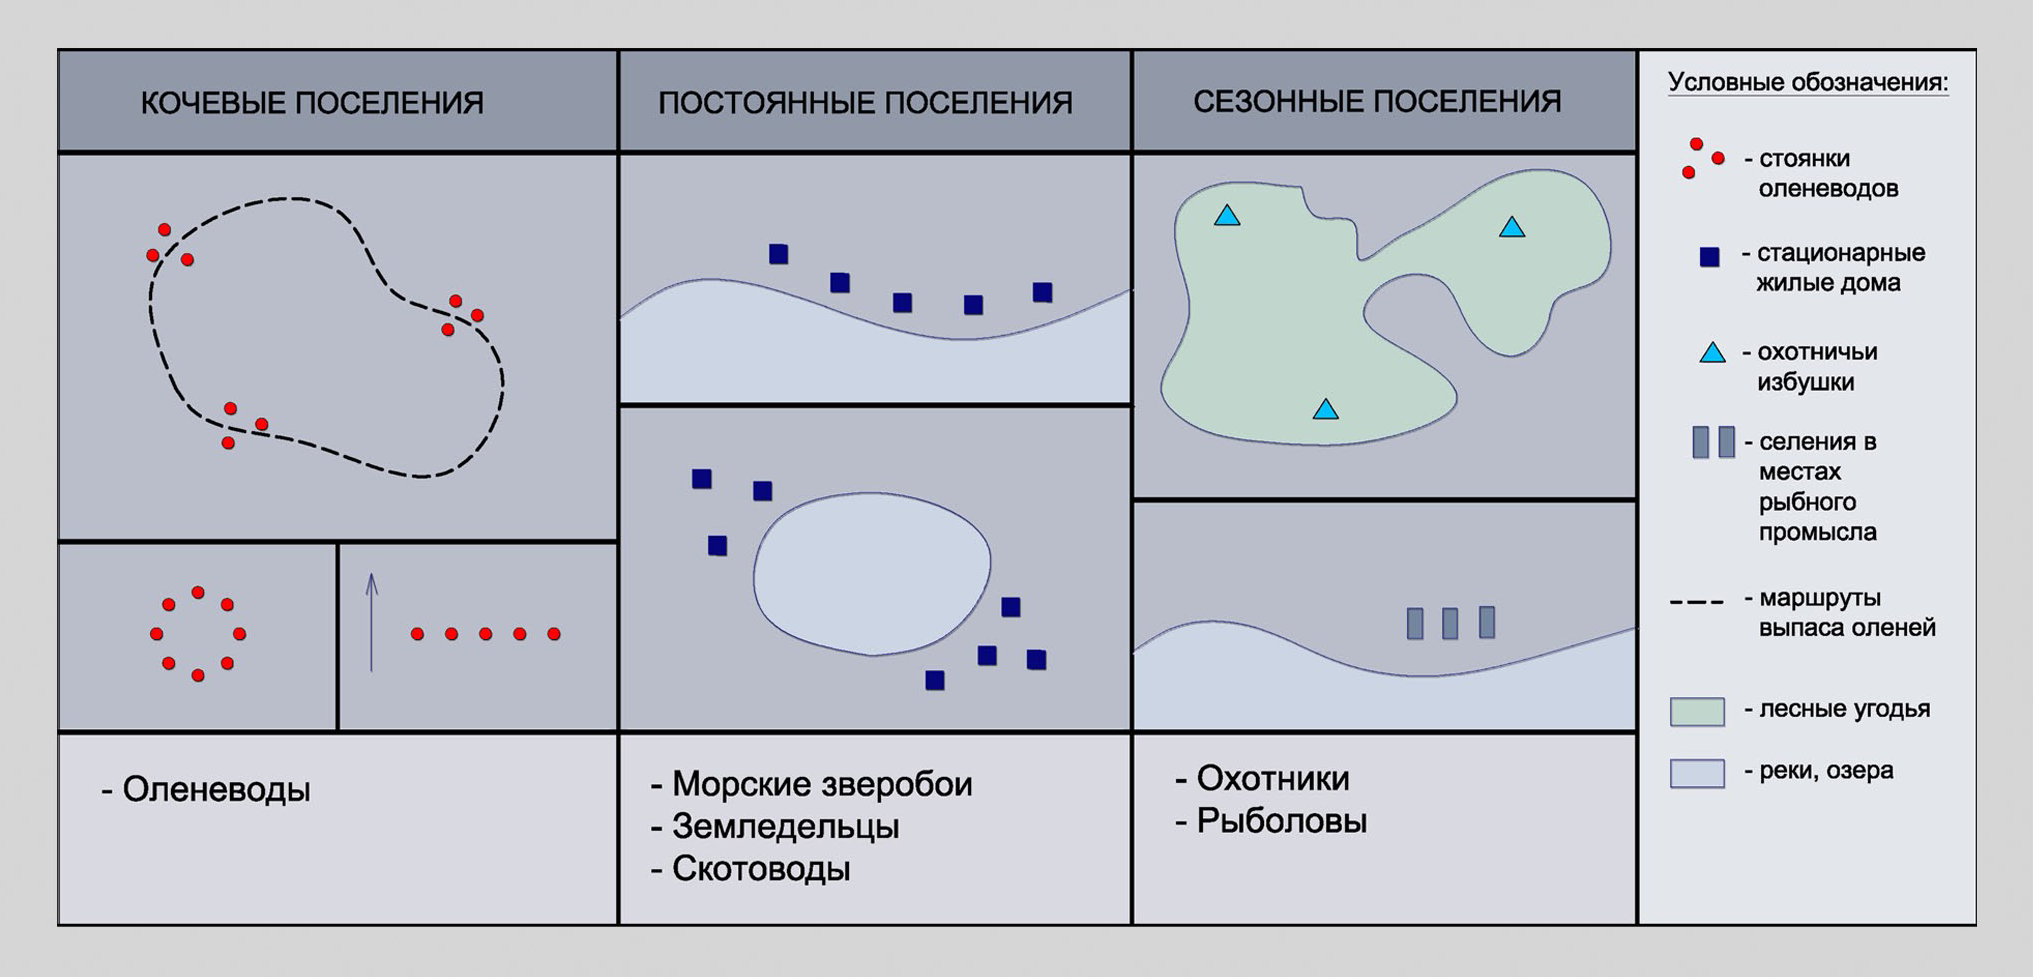
\includegraphics[width=\textwidth]{assets/figures/ch01_s10_urbanplan_settelsystems03}
    \caption{Типы традиционных поселений коренных народов Севера (графика разработана Благодетелевой О.М.)}
    \author{графика разработана Благодетелевой О.М.}
    \label{fig:ch01_s10_urbanplan_settelsystems03}
  \end{figure}